\documentclass[a4paper, 12pt]{memoir}

\usepackage[utf8]{inputenc}
\usepackage[T1]{fontenc}
\usepackage[a4paper]{geometry}
\geometry{verbose,tmargin=2.5cm,bmargin=2.5cm,lmargin=2.5cm,rmargin=2.5cm}
\pagestyle{Ruled}
\usepackage{array}
\usepackage{verbatim}
\usepackage{prettyref}
\usepackage{booktabs}
\usepackage{textcomp}
\usepackage{url}
\usepackage{amsmath}
\usepackage{graphicx}
\usepackage{amssymb}
\usepackage[usenames,dvipsnames]{xcolor}

\usepackage[spanish]{babel}
\addto\shorthandsspanish{\spanishdeactivate{~<>}}

\usepackage{mathpazo}%Letra palatino con fuentes para matemáticas


%\usepackage{biblatex}
%\usepackage{csquotes}

\usepackage{amsfonts}

\usepackage{memhfixc}
\usepackage{mempatch}
\raggedbottom
\sloppybottom
\clubpenalty=10000
\widowpenalty=10000

\newcommand{\HRule}{\rule{\linewidth}{0.7mm}}

\pretitle{\vfill \begin{center} \HRule \par \bfseries \scshape \HUGE}
\posttitle{\HRule \par\end{center}}

\preauthor{\begin{center} \large \scshape}
\postauthor{\par\end{center}}

%\date{}
\predate{\vfill \begin{center}\large\scshape}
\postdate{\par\end{center}\vfill}



\openany
\chapterstyle{southall}

\makepagestyle{index}
    \makeheadrule{index}{\textwidth}{\normalrulethickness}
    \makeevenhead{index}{\rightmark}{}{\leftmark}
    \makeoddhead{index}{\rightmark}{}{\leftmark}
    \makeevenfoot{index}{\thepage}{}{}
    \makeoddfoot{index}{}{}{\thepage}

\makeindex
\makeindex[inst]

\usepackage{hyperref}
\hypersetup{
    bookmarks=true,         % show bookmarks bar?
    unicode=true,          % non-Latin characters in Acrobat’s bookmarks
    bookmarksnumbered=true,
    bookmarksopen=false,
    breaklinks=true,
    backref=true,
    pdftoolbar=true,        % show Acrobat’s toolbar?
    pdfmenubar=true,        % show Acrobat’s menu?
    pdffitwindow=false,     % window fit to page when opened
    pdfstartview={FitH},    % fits the width of the page to the window
    pdftitle={Libro de Resumenes}
    pdfauthor={Comités Organizador y Científico}
    pdfsubject={R},   % subject of the document
    pdfcreator={AucTeX/Emacs},   % creator of the document
    pdfproducer={LaTeX}, % producer of the document
    pdfnewwindow=true,      % links in new window
    pdfborder={0 0 0},
    colorlinks=true,       % false: boxed links; true: colored links
    linkcolor=Brown,          % color of internal links
    citecolor=BrickRed,        % color of links to bibliography
    filecolor=black,      % color of file links
    urlcolor=Blue           % color of external links 
}


\usepackage[sectionbib]{chapterbib}
\usepackage[plain, spanish, noabstract, sort, nonamereplace]{flexbib}
\bibpunct{[}{]}{,}{n}{}{;} %comandos de natbib: separadores [], etc


\newcommand{\com}[1]{%
\begin{center}
  \textsc{%
    \href{http://r-es.org/tiki-download_file.php?fileId=#1}{Comunicación
      (pdf)}}
\end{center}
}

\newcommand{\taller}[1]{%
\begin{center}
  \textsc{%
    \href{http://r-es.org/tiki-download_file.php?fileId=#1}{Material}}
\end{center}
}


\setcounter{tocdepth}{0}

\begin{document}

\frontmatter

\begin{titlingpage}

  \title{
    \Large{Libro de Resúmenes}\\
    \Huge{V Jornadas de Usuarios de R}\\
    \vspace{15pt}
    \Large{Centro de Arte y Tecnología ETOPIA, Zaragoza}\\
    \large{12 y 13 de Diciembre de 2013}\\
  }

  \author{
    Comités Organizador y Científico\\
    \texttt{http://r-es.org/5j}}

  \date{1 de Diciembre de 2013}

  \maketitle


\end{titlingpage}



% \chapterprecis{\vfill{}
% }

% \rule[.5ex]{\linewidth}{1pt} 

% El orden de las ponencias recogido en este documento no está
% relacionado con el orden de presentación en las Jornadas.

% \rule[.5ex]{\linewidth}{1pt} 

% \vfill
\vspace*{\fill}




\rule[.5ex]{\linewidth}{1pt} 
© 2013 Organización de las V Jornadas de Usuarios de R

\begin{center}

\includegraphics[scale=0.5]{Logos/cc-logo}
\par\end{center}

Esta obra está bajo una licencia \textbf{Reconocimiento-No comercial-Compartir
bajo la misma licencia} 3.0 España de Creative Commons. Para ver una
copia de esta licencia, visite:\\
 \url{http://creativecommons.org/licenses/by-nc-sa/3.0/es/legalcode.es}.

Usted es libre de copiar, distribuir y comunicar públicamente la obra,
y hacer obras derivadas bajo las condiciones siguientes:
\begin{itemize}
\item 
\includegraphics[scale=0.35]{Logos/by} \textbf{Reconocimiento}.
Debe reconocer los créditos de la obra de la manera especificada por
el autor o el licenciador (pero no de una manera que sugiera que tiene
su apoyo o apoyan el uso que hace de su obra). 
\item 
\includegraphics[scale=0.35]{Logos/nc-eu} \textbf{No comercial}.
No puede utilizar esta obra para fines comerciales. 
\item 
\includegraphics[scale=0.35]{Logos/sa} \textbf{Compartir bajo la
misma licencia}. Si altera o transforma esta obra, o genera una obra
derivada, sólo puede distribuir la obra generada bajo una licencia
idéntica a ésta. 
\end{itemize}
Al reutilizar o distribuir la obra, tiene que dejar bien claro los
términos de la licencia de esta obra. Alguna de estas condiciones
puede no aplicarse si se obtiene el permiso del titular de los derechos
de autor. Nada en esta licencia menoscaba o restringe los derechos
morales del autor.



\cleardoublepage

\tableofcontents

\cleardoublepage

\part{Información General}

\textbf{TODO: Vas por aquí}
\chapter{Presentación}

Las V Jornadas de Usuarios de R tendrán lugar en el
\href{http://www.zaragoza.es/ciudad/idezar/detalle_Centro?id=5105}{Etopia-Centro
  de Arte y Tecnología de Zaragoza}, los días 12 y 13 de diciembre de
2013. Etopia es un centro de creatividad, innovación y emprendimiento,
16.000 m2 para el trabajo colaborativo, la búsqueda de nuevos caminos
y para aprender haciendo y compartiendo. Forma parte de la
\href{http://www.zaragoza.es/ciudad/sectores/tecnologia/milladigital.htm}{Milla
  Digital de Zaragoza}, promovida por el
\href{http://www.zaragoza.es/ciudad/sectores/tecnologia/}{Área de
  Tecnología del ayuntamiento de Zaragoza}.

Las jornadas, como no podría ser de otra forma, van a incluir trabajos
de todos los ámbitos y están abiertas tanto a usuarios como a
entusiastas de R independientemente de su área de interés. Los
objetivos para estas jornadas serán los mismos que para las anteriores
que tan buenos resultados obtuvieron. Estos objetivos incluyen:

\begin{itemize}
\item Proporcionar un punto de encuentro a los usuarios de R 
\item Fomentar la colaboración entre ellos en un ambiente multidisciplinar 
\item Divulgar el conocimiento del lenguaje y sus posibilidades 
\item Promover el uso de R 
\end{itemize}

Usuarios y entusiastas de R de todos los ámbitos —universidad,
institutos de investigación, administraciones públicas, empresa
privada— están invitados a participar en las V Jornadas y compartir
con la comunidad aplicaciones y ejemplos interesantes que reflejen la
madurez de R y la diversidad de los problemas y campos en los que
viene utilizándose con éxito. Existen las siguientes modalidades de
participación:
\begin{itemize}
\item Comunicaciones orales de 15 minutos seguidas de una discusión de
  5 minutos (la decisión sobre la duración podría sufrir
  modificaciones en función del número final de ellas).

\item Presentaciones breves de 5 minutos, donde el ponente expone en
  tres diapositivas (número orientativo) de forma breve y concisa,
  quién es/son, qué ha/n hecho, y qué resultados y conclusiones se
  extraen de ello que puedan ser de interés para otras personas.

\item Talleres de 2 horas aproximadamente, donde se explican paquetes,
  procedimientos, y programas de R.  En esta edición, además de las
  ponencias invitadas, las presentaciones orales y los talleres, se
  llevarán a cabo presentaciones breves donde el ponente expondrá de
  forma concisa los resultados y conclusiones de alguna investigación
  llevada a cabo con R que puedan ser de interés para otros colegas.
\end{itemize}

Desde el comité organizador nos gustaría destacar la excelente labor
llevada a cabo por el comité científico, a los ponentes de los
talleres y a todos los asistentes que han permitido confeccionar el
programa que a continuación detallamos y esperamos que sea de vuestro
interés.

Esperamos que las jornadas resulten lo más provechosas posibles y que
disfrutéis de una confortable estancia en Zaragoza.


\chapter{Información útil}

\section{Ubicación de las jornadas}

Las jornadas se celebrarań en el Centro de Arte y Tecnología 
\href{http://www.zaragoza.es/ciudad/idezar/detalle_Centro?id=5105}{CAT-ETOPIA}
que  el Ayuntamiento de Zaragoza ha desarrollado en la llamada 
\href{http://www.milladigital.es/espanol/home.php}{Milla Digital}. 

\begin{center}

\includegraphics[width=0.6\textwidth]{Logos/logoMillaAyZgz.png}
\end{center}

El C.A.T. está situado prácticamente en el centro de la Milla Digital, 
justo enfrente de la Estación de Delcias.  se encuentra comunicado con 
centro de la ciduad (Puerta del Carmen y Palza del Paraiso) mediante las 
lineas de autobuses
\href{http://www.urbanosdezaragoza.es/frm_verdescarga.php?ref=175}{34 y 52},
también pueden resultar de interés las lineas circulares
\href{http://www.urbanosdezaragoza.es/frm_verdescarga.php?ref=175}{Ci1 y Ci2}.

\begin{center}
\textbf{** TODO: mapa paradas}. 
% 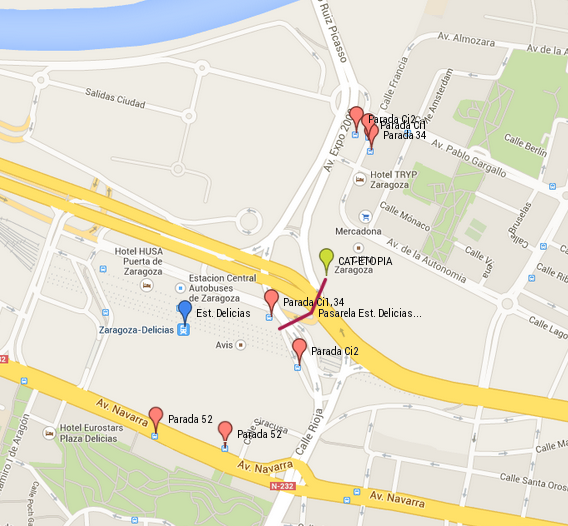
\includegraphics[width=0.6\textwidth]{Logos/mapaParadas.png}
\end{center}

Las comunicaciones orales y breves se llevarán a cabo en el auditorio 
del William J. Mitchell CAT-ETOPIA. Para acceder al edificio cada 
participante se deberá identificar en recepción donde disponen de una 
lista con todos los asistentes.


\section{Talleres}

Los participantes a los talleres deben traer su propio ordenador portátil 
con las herramientas que indiquen los responsables de los talleres. La 
inscripción a los talleres se realizará en el momento de la entrega de
material, en el momento de la recepción de los participantes. Dado el 
limitado número de plazas, se reservará plaza por orden de inscripción. 
Los talleres se desarrollarán en las aulas de que dispone el CAT-ETOPIA 
para laboratorios audiovisuales y meetings.


\section{Certificados}
\textbf{...Esto está por decidir}
Los certificados se enviarán por correo electrónico una vez pasadas
las Jornadas.  

\section{Material}

Todo el material, está disponible a través de la página web de las Jornadas 
\href{http://r-es.org/V+Jornadas}. 



\chapter{Comité organizador}

\begin{itemize}

\item \href{http://www.datanalytics.com}{J. Gil Bellosta} (coordinador)
\item \href{http://www.scien-analytics.com}{Sergio Jiménez} (Scien Analytics)
\item Luis Mariano Esteban (U. de Zaragoza)
\item \href{http://www.scien-analytics.com}{Rubén Moreno Ruíz} (Scien Analytics)
\item \href{[http://www.scien-analytics.com}{Miguel Ángel Luzón} (Scien Analytics)
\item Jorge Ojeda (U. de Zaragoza)
\item \href{http://ueb.vhir.org|Vall d'Hebron Research Institute}{Xavier de Pedro Puente}
\item  Emilio Torres Manzanera (U. de Oviedo)
\end{itemize}

\chapter{Comité científico}


\begin{itemize}

\item Sandra Barragán
\item Ramón Díaz-Uriarte
\item Juan Ramon González
\item \href{http://oscarperpinan.github.io}{Oscar Perpiñán}
\item Miguel Angel Rodríquez (coordinador)
\item Isaac Subirana
\item Joan Vila
\item \href{http://www.ottofwagner.es}{Otto F. Wagner}

\end{itemize}


\chapter{Patrocinadores}



\begin{center}


\includegraphics[width=0.33\textwidth]{Logos/logoMillaAyZgz.png}
\hspace{1cm}


\includegraphics[width=0.33\textwidth]{Logos/logoEtopia.jpg}
\hspace{1cm}


\includegraphics[width=0.33\textwidth]{Logos/logoScien.png}
\hspace{1cm}


\includegraphics[width=0.33\textwidth]{Logos/logoComRHisp.png}
\vspace{1cm}


\includegraphics[width=0.33\textwidth]{Logos/logoRevolAnal}
\hspace{1cm}


\includegraphics[width=0.33\textwidth]{Logos/logoUZ.png}
\hspace{1cm}


\includegraphics[width=0.33\textwidth]{Logos/logoSynergic.png}
\vspace{1cm}


\includegraphics[width=0.33\textwidth]{Logos/logoTelefID.png}

\end{center}


\chapter{Programa}

% \begin{itemize}
\item \textsc{\textbf{JUEVES 15 DE NOVIEMBRE}}
  \begin{itemize}

  \item 09:00-09:30 Acreditación y recogida de información

  \item 09:30-09:45 Inauguración oficial de las Jornadas. J.R. González.

  \item 09:45-10:30 Conferencia Inaugural.  J. Vila:
    \href{http://r-es.org/tiki-download_file.php?fileId=484}{Enseñando
      estadística: como mejorar los conocimientos utilizando R
      para la creación de prácticas individualizadas.}
  \item 10:30-12:00 Sesión de Comunicaciones (I) Moderador: G.R
    Serrano
    \begin{itemize}
    \item 10:30-10:45 C. E. Melo Funciones geoestadísticas y
      funciones de base radial en el programa R: Paquete geospt
    \item 10:45-11:00 E. L. Cano Investigación operativa
      reproducible. Aplicación a la optimización de sistemas
      energéticos
    \item 11:00-11:15 C. J. Gil MicroDatosEs: un paquete para leer
      ficheros de microdatos públicos
    \item 11:15-11:30 A. Alabert Flujo de trabajo reproducible con
      R
    \item 11:30-11:45 N. Longford A study of poverty and income
      inequality in the EU countries
    \end{itemize}
  \item 12:00-12:30 Café
 
  \item 12:30-14:00 Sesión de Comunicaciones (II) Moderador:
    A. Sánchez
    \begin{itemize}
    \item 12:30-12:45 R. Pazmiño Caracterizacion del software
      estadistico en las escuelas de estadistica del
      Ecuador. Enfoque en el software R
    \item 12:45-13:00 O. Ivina A cross-country air quality
      analysis using R

    \item Comunicaciones Breves
      \begin{itemize}
      \item 13:00-13:07 M. Sánchez Inferencia estadística para el
        equilibrio de Hardy-Weinberg en estudios de genotipado con
        Missing Data
      \item 13:07-13:15 I. Roman Representación de las Dinámicas
        de Precios Hoteleros mediante R
      \item 13:15-13:22 D. Moriña El paquete complex.surv.dat.sim
        de R: Simulación de datos de supervivencia complejos
      \item 13:22-13:30 J-L. Cañadas De Excel a html utilizando
        knitr + markdown + googleVis . Un ejemplo
      \item 13:30-13:37 B. González Programación Lineal y
        Programación Dinámica con R
      \item 13:37-13:45 A. Sanz-García Selección de variables y
        modelizado predictivo en R
      \item 13:45-13:52 F. Antoñanzas-Torres Evaluación de modelos
        paramétricos de predicción de irradiación global solar
        mediante variables meteorológicas típicas
      \item 13:52-14:00 R. Fernández Uso de métodos de
        interpolación espacial para la predicción de variables en
        entornos vitivinícolas
      \end{itemize}
    \end{itemize}

  \item 14:00-16:00 Comida
  \item 16:00-17:45 Talleres (I)
    \begin{itemize}
    \item G. R. Serrano Web scraping con R
    \item F. Carmona Informes dinámicos con LaTeX y R: utilización
      de Sweave y knitr.
    \end{itemize}

  \item 17:45-18:15 Café
  \item 18:15-20:00 Talleres (II)
    \begin{itemize}
    \item X. de Pedro Interfaces Web 2.0 para R con Tiki
    \item A. Sánchez Edición (y mucho más) potente en R con ESS
      ("Emacs Speaks Statistics")
    \end{itemize}
  \item 20:00-21:00 Asamblea Asociación “Comunidad R-Hispano”

  \item 21:30 Cena

  \end{itemize}
 

 

\item \textsc{\textbf{VIERNES 16 DE NOVIEMBRE}}

  \begin{itemize}
  \item 10:00-11:00 Sesión de Comunicaciones (III) Moderador:
    F. Carmona
    \begin{itemize}
    \item 10:00-10:15 A. Lobo R como caja de herramientas para SIG
      y Teledetección: reflexiones a partir de experiencias
    \item 10:15-10:30 V. Urrea Gales Simulación de perfiles
      genéticos de riesgo
    \item 10:30-10:45 A. Urkaregi Construcción de un Índice Global
      de Valoración
    \item 10:45-11:00 G. Estévez-Pérez kerdiest: An R Package for
      Distribution Function Estimation and Applications
    \end{itemize}

  \item 11:00-12:00 Sesión de Comunicaciones (IV) Moderador:
    Ll. Ramon
    \begin{itemize}
    \item 11:00-11:15 N. M. Villanueva seq2R: Detección de puntos
      de cambio en secuencias genómicas
    \item 11:15-11:30 J Graffelman Exploring bi-allelic genetic
      markers with the HardyWeinberg package
    \item 11:30-11:45 M. Sestelo FWDselect: Selección de variables
      en modelos de regresión
    \item 11:45-12:00 B. Santos Reducción unidimensional de 12
      items de la Escala de sobrecarga de Zarit en cuidadores de
      pacientes con demencia mediante teoría de respuesta a los
      ítems.
    \item 12:00-12:15 J. Barrera The optimal Allocation package
      for longitudinal studies design with time-varying esposure
    \end{itemize}
  	 
  \item 12:15-12:45 Café

  \item 12:45-14:30 Talleres (III)
    \begin{itemize}
    \item A. Karatzoglou Machine learning in R
    \end{itemize}


  \item 14:30-16:15 Comida
  \item 16:15-18:00 Talleres (IV)
    \begin{itemize}
    \item A. Ruiz Introducción a las Reference Classes
      (programación orientada a objetos en R)
    \item Ll. Ramon, R. Borras y A. Vall Introducción práctica a
      la librería ggplot2 y su integración con ggmap
    \end{itemize}
  \item 18:00-18:30 Café

  \item 18:30-19:00 Clausura Oficial de las IV Jornadas

  \end{itemize}
\end{itemize}






\mainmatter

\renewcommand{\partname}{}

\part{Sesión de Comunicaciones Jueves}
\label{part:comunicacionesI}

\chapter{Evaluación del uso de modelos mixtos para estimación de la tasa de paro con poca muestra}

\chapterprecis{José Luis Cañadas Reche\\Técnico de Investigación en el Instituto de Estudios Sociales Avanzados (IESA-CSIC)}

\index{Luis Cañadas Reche, José}

\index[inst]{Técnico de Investigación en el Instituto de Estudios Sociales Avanzados (IESA-CSIC)}

La EPA, a pesar de ser la mayor encuesta de España, no ofrece muestra suficiente para algunas desagregaciones, tal es el caso por ejemplo, si queremos estimar la tasa de paro de los hombres de 35 a 40 años residentes en Zaragoza y con estudios universitarios.

El uso de modelos mixtos se ha utilizado tradicionalmente para modelar estructuras de covarianzas no contempladas por los modelos lineales tradicionales. Los modelos mixtos, sin embargo, también pueden ser utilizados para obtener unas estimaciones más precisas de las medias condicionales.

Para comprobarlo, se utilizó R para comparar la estimación clásica con la obtenida mediante modelos mixtos. Se tomaron diversas 5 submuestras de la EPA de diferente tamaño. Se calculó la tasa de paro a nivel provincial mediante ambos métodos repitiendo el proceso 200 veces, obteniendo como medida de precisión el error absoluto medio. Los modelos mixtos dieron un menor EAM incluso para muestras inferiores al 5% de la encuesta.


%\bibliographystyle{plain}

%\bibliography{resumenes/evaluacion_del_uso_de_modelos_mixtos_para_estimacion_de_la_tasa_de_paro_con_poca_muestra}

\chapter{Package xkcd: Plotting ggplot2 graphics in a XKCD style}

\chapterprecis{Emilio Torres Manzanera\\Universidad de Oviedo}

\index{Torres Manzanera, Emilio}

\index[inst]{Universidad de Oviedo}

Se presenta el paquete xkcd, que realiza gráficos ggplot2 como si fueran trazados a mano, siguiendo el estilo de las tiras cómicas de XKCD.

%\bibliographystyle{plain}

%\bibliography{resumenes/package_xkcd__plotting_ggplot2_graphics_in_a_xkcd_style}

\chapter{Desarrollo de Interfaces Web utilizando programación funcional en R}

\chapterprecis{Jorge~Luis Ojeda Cabrera\\Dept- Métodos Estadísticos, Univ. de Zaragoza}

\index{Ojeda Cabrera, Jorge~Luis}

\index[inst]{Dept- Métodos Estadísticos, Univ. de Zaragoza}

  Este trabajo muestra el desarrollo de interfaces web para funciones en R mediante las ideas utilizadas en el paquete 'miniGUI'. Tanto en dicho paquete como en este trabajo se propugna el uso de las capacidades de R para desarrollar programación funcional y 'calcular sobre el lenguaje' a fin de disociar el código necesario para desarrollar los  cálculos puramente estadísticos del código utilizado en la construcción de la interfaz 
de usuario. Esto no sólo ayuda al desarrollo rápido de aplicaciones web, sino que permite separar convenientemente y de una forma sencilla la construcción del Interfaz de la funcionalidad estadística, proporcionando además completa flexibilidad a la hora de desarrollar los interfaces.

  En este caso se desarrollan Interfaces Web para el usuario (WUI)en HTML para 
funciones R que permiten la introducción de los datos mediante formularios HTML. 
El paquete ha sido probado con la utilidad CGI R FastRWeb y con la aplicación 
web sumo con configuración básica.

  El desarrollo de este trabajo se concreta de momento en una versión incompleta
del paquete miniHtmlWUI en la que se implementan todas estas ideas junto 
con algunos ejemplos básicos de la misma.  

%\bibliographystyle{plain}

%\bibliography{resumenes/desarrollo_de_interfaces_web_utilizando_programacion_funcional_en_r}

\chapter{Métrica de Wasserstein para la comparación de matrices origen-destino}

\chapterprecis{Aleix Ruiz de Villa, Jordi Casas, Martijn Breen\\TSS - Transport Simulation Systems\\RugBcn, Grupo de usuarios de Barcelona}

\index{Ruiz de Villa, Aleix}
\index{Casas, Jordi}
\index{Breen, Martijn}

\index[inst]{TSS - Transport Simulation Systems}
\index[inst]{RugBcn, Grupo de usuarios de Barcelona}

Las matrices origen-destino (OD) son un elemento básico en los estudios de tráfico. Dada una red de transporte (por ejemplo una autopista con sus vías secundarias), describen el número de viajes que se dan en un intervalo de tiempo, donde los orígenes y destinos pertenecen a un conjunto fijo de localizaciones, llamados centroides.

El problema que abordamos aquí es el de comparar dos matrices OD. En un principio, se pueden ver las diferencias celda a celda. Sin embargo, esta comparación no recoge la topología del red. Es decir, dos centroides muy cercanos pueden tener viajes muy diferentes, debido por ejemplo a las perturbaciones del proceso de muestreo, pero en esencia ambas matrices recoger el mismo tipo de información.

Para abordar dicho problema, utilizamos técnicas de transporte de masas, una rama teórica de las matemáticas, íntimamente relacionada con problemas de transporte. Dados dos pares od (o1,d1) y (o2,d2), definimos la distancia entre ellos, como el tiempo de transporte (calculado en base a la topología de la red) necesario para desplazarse de un origen al otro y volver del correspondiente destino: es decir d(o1,o2) + d(d2,d1). Bajo estas circumstancias, definimos (informalmente) la distancia entre matrices od, como el mínimo tiempo de desplazamiento para mover la masa total de la matriz (número total de viajes) od1 hasta od2 y luego devolverla. En transporte de masas, esta distancia es conocida como la distancia de Wasserstein. Este problema se resuelve mediante técnicas básicas de programación lineal.

El principal interés de este método, es que creemos que se puede utilizar en otras áreas científicas como el estudio de movimientos demográficos o el estudio de redes de telecomunicaciones y que podría tener aplicaciones peculiares como la comparación de ofertas de vuelo de dos compañías aereas. Para ello desarrollamos un paquete en R, que permita fácilmente el cálculo de dicha distancia.

%\bibliographystyle{plain}

%\bibliography{resumenes/metrica_de_wasserstein_para_la_comparacion_de_matrices_origen_destino}

\chapter{Categorización automática de contenidos web con R}

\chapterprecis{Pedro Concejero, César García, Ana Armenta, Paulo Villegas, J. Gregorio Escalada, \\Telefónica Digital, Product Development and Innovation}

\index{Concejero, Pedro}
\index{García, César}
\index{Armenta, Ana}
\index{Villegas, Paulo}
\index{Gregorio Escalada, J.}
\index{, NA}

\index[inst]{Telefónica Digital, Product Development and Innovation}

Telefónica Digital – PDI ha desarrollado un diccionario de contenidos web tomando como base la jerarquía temática y las clasificaciones del Open Directory Project, también conocidas como DMoz –por directory.mozilla (http://www.dmoz.org/). Se trata de un proyecto colaborativo abierto y multilingüe, en el que editores voluntarios listan y categorizan enlaces a páginas web. Muchos creadores de contenidos web categorizan los mismos en dmoz con el fin de obtener una buena posición en los buscadores, pues muchos de ellos utilizan este directorio como semilla para realizar el crawling de Internet completo
Dos limitaciones importantes de esta taxonomía son su cobertura limitada, esto es, el contenido que no ha sido clasificado en DMoz, y su estructura desbalanceada (la profundidad de la jerarquía y su densidad es muy variable por categorías). Resulta por tanto interesante plantearse un proceso que pueda proporcionar la categoría o clasificación de un contenido web de forma automática, tomando como input el texto completo obtenido de webs reales mediante un crawler, sobre un subconjunto más balanceado de la jerarquía del ODP. Esta presentación describirá el proceso completo que comienza con el análisis de logs representativos de navegación web de usuarios, con el objetivo de seleccionar las categorías más populares o significativas, para luego extraer automáticamente el contenido (texto) completo de las páginas webs asignadas a estas categorías. 
La extracción de contenido web (crawl) se realizó mediante nutch (un módulo de apache), al que se le pasaron un total de 10658 dominios que tienen un número mínimo de visitas.  Sin embargo, no podemos extraer automáticamente el texto de todos los dominios que le pasemos, debido a errores tipo “Forbidden” (la web destino no permite la extracción de texto) o “Service unavailable” (el servidor web destino no funciona).  De hecho la selección final, esto es, dominios de los que dispondremos de texto completo (con profundidad 1) y de su categoría DMoz, se reduce a 4072. 
Un proceso de identificación de idioma –mediante tecnología desarrollada por el grupo de Tecnología del Habla de Telefónica I+D- permite seleccionar cuáles de ellos se utilizarán, en principio castellano, catalán y gallego –filtrando por tanto inglés y euskera entre otros. La figura a continuación muestra el número de dominios finalmente disponible para entrenamiento por categoría DMOZ (imponiendo como requisito al menos 10 dominios por categoría), en total 2283 páginas correspondientes a 44 categorías, que sigue la típica  distribución de ley de potencia. Sitios web de noticias (periódicos pero también revistas y publicaciones electrónicas, portales y lugares de desarrollo web) son las categorías con mayor  número de dominios clasificados como pertenecientes a ellas en el diccionario DMOZ, seguidos por negocios, sitios de la Administración Pública y la categoría de automóvil.
Este texto será después pre-procesado con la librería tm, y se utilizará la implementación del algoritmo de Porter de la librería SnowBall como stemmer. El objetivo es obtener una matriz de frecuencias de raíces de palabras, así como posiblemente bigramas, por categoría.
Estas webs, o dominios, se dividen en un conjunto de entrenamiento y otro de test, de forma aleatoria, en proporción 80/20 respectivamente, para entrenar y validar clasificadores estadísticos.
Los conjuntos creados se aplican a los algoritmos de clasificación incluidos en la librería RTextTools .RTextTools facilita además enormemente la medición de precisión y otros indicadores de rendimiento de cada uno de los algoritmos probados. La comunicación oral presentará todos los resultados obtenidos en este trabajo. 
La lista a continuación muestra los resultados preliminares de dos de los algoritmos incluidos en RTextTools, sin que el texto haya sido tratado por el stemmer debido a problemas técnicos con la librería Snowball –que serán solucionados lo antes posible y sin duda antes de la conferencia. 
Los algoritmos que no están en la lista es porque no son aplicables o han dado error en esta primera prueba (a menudo debido a desbordamiento de memoria). La lista muestra el tiempo necesario para el cómputo del modelo en un servidor MS-Windows Server 2003 x64, con procesador Quad-Core AMD Opteron y 30 GB de RAM, así como la precisión. Esta medida es, más concretamente, la proporción promedio (para todas las categorías) con la que el algoritmo predice que un dominio del conjunto de validación pertenece a la clase en la que realmente está clasificado. Esto es, proporción de clasificaciones correctas promediada para todo el conjunto de textos contenido en el conjunto de validación. 
Support Vector Machines (SVM) – 48.43 segundos – 0.621 (proporción de aciertos promedio)
Maximum Entropy (MAXENT) – 22.15 minutos – 0.714 (proporción de aciertos promedio)

REFERENCIAS (en formato estándar):
Feinerer, I. (2010). Introduction to the tm Package Text Mining in R, 1–7. Retrieved from http://cran.r-project.org/web/packages/tm/vignettes/tm.pdf
Ingersoll, G. S., Morton, T. S., & Farris, A. L. (2013). Taming Text: How to find, organize and manipulate it. New York: Manning.
Jurka, A. T. P., Collingwood, L., Boydstun, A. E., Gross-, E., & Atteveldt, W. Van. (2013). Package “ RTextTools .” Retrieved from http://cran.r-project.org/web/packages/RTextTools/RTextTools.pdf
Jurka, T. P., Collingwood, L., Boydstun, A. E., Grossman, E., & Van, W. (2013). RTextTools : A Supervised Learning Package for Text Classification. The R Journal, 5, 6–12. Retrieved from http://journal.r-project.org/archive/2013-1/collingwood-jurka-boydstun-etal.pdf
Qi, X., & Davison, B. D. (2009). Web Page Classification : Features and Algorithms ∗. ACM Computing Surveys, 41(June), 1–31. Retrieved from http://www.cse.lehigh.edu/~xiq204/pubs/classification-survey/LU-CSE-07-010.pdf
Radovanovic, M., & Ivanovi, M. (2008). TEXT MINING : Bag-of-Words Document Representation Machine Learning with Textual Data. Novi Sad Journal of Mathematics, 38(3), 227–234.



%\bibliographystyle{plain}

%\bibliography{resumenes/categorizacion_automatica_de_contenidos_web_con_r}

\chapter{Mejora de la detección visual de datos atípicos mediante una modificación en las caras de Chernoff}

\chapterprecis{Beatriz González Pérez, Victoria López López, Jorge Cordero\\Universidad Complutense de Madrid}

\index{González Pérez, Beatriz}
\index{López López, Victoria}
\index{Cordero, Jorge}

\index[inst]{Universidad Complutense de Madrid}

En este trabajo se realiza una mejora de la función de R que construye el gráfico de las caras de Chernoff para un perfil multivariante. Esta mejora se realiza mediante una categorización utilizando una paleta de colores y se aplica a una base de datos real. El procedimiento proporciona al investigador una mayor capacidad visual a la hora de detectar datos atípicos.

%\bibliographystyle{plain}

%\bibliography{resumenes/mejora_de_la_deteccion_visual_de_datos_atipicos_mediante_una_modificacion_en_las_caras_de_chernoff}

\chapter{Categorización automática de contenidos web con R}

\chapterprecis{Pedro Concejero, César García, Ana Armenta, Paulo Villegas, J. Gregorio Escalada, \\Telefónica Digital, Product Development and Innovation}

\index{Concejero, Pedro}
\index{García, César}
\index{Armenta, Ana}
\index{Villegas, Paulo}
\index{Gregorio Escalada, J.}
\index{, NA}

\index[inst]{Telefónica Digital, Product Development and Innovation}

Telefónica Digital – PDI ha desarrollado un diccionario de contenidos web tomando como base la jerarquía temática y las clasificaciones del Open Directory Project, también conocidas como DMoz –por directory.mozilla (http://www.dmoz.org/). Se trata de un proyecto colaborativo abierto y multilingüe, en el que editores voluntarios listan y categorizan enlaces a páginas web. Muchos creadores de contenidos web categorizan los mismos en dmoz con el fin de obtener una buena posición en los buscadores, pues muchos de ellos utilizan este directorio como semilla para realizar el crawling de Internet completo
Dos limitaciones importantes de esta taxonomía son su cobertura limitada, esto es, el contenido que no ha sido clasificado en DMoz, y su estructura desbalanceada (la profundidad de la jerarquía y su densidad es muy variable por categorías). Resulta por tanto interesante plantearse un proceso que pueda proporcionar la categoría o clasificación de un contenido web de forma automática, tomando como input el texto completo obtenido de webs reales mediante un crawler, sobre un subconjunto más balanceado de la jerarquía del ODP. Esta presentación describirá el proceso completo que comienza con el análisis de logs representativos de navegación web de usuarios, con el objetivo de seleccionar las categorías más populares o significativas, para luego extraer automáticamente el contenido (texto) completo de las páginas webs asignadas a estas categorías. 
La extracción de contenido web (crawl) se realizó mediante nutch (un módulo de apache), al que se le pasaron un total de 10658 dominios que tienen un número mínimo de visitas.  Sin embargo, no podemos extraer automáticamente el texto de todos los dominios que le pasemos, debido a errores tipo “Forbidden” (la web destino no permite la extracción de texto) o “Service unavailable” (el servidor web destino no funciona).  De hecho la selección final, esto es, dominios de los que dispondremos de texto completo (con profundidad 1) y de su categoría DMoz, se reduce a 4072. 
Un proceso de identificación de idioma –mediante tecnología desarrollada por el grupo de Tecnología del Habla de Telefónica I+D- permite seleccionar cuáles de ellos se utilizarán, en principio castellano, catalán y gallego –filtrando por tanto inglés y euskera entre otros. La figura a continuación muestra el número de dominios finalmente disponible para entrenamiento por categoría DMOZ (imponiendo como requisito al menos 10 dominios por categoría), en total 2283 páginas correspondientes a 44 categorías, que sigue la típica  distribución de ley de potencia. Sitios web de noticias (periódicos pero también revistas y publicaciones electrónicas, portales y lugares de desarrollo web) son las categorías con mayor  número de dominios clasificados como pertenecientes a ellas en el diccionario DMOZ, seguidos por negocios, sitios de la Administración Pública y la categoría de automóvil.
Este texto será después pre-procesado con la librería tm, y se utilizará la implementación del algoritmo de Porter de la librería SnowBall como stemmer. El objetivo es obtener una matriz de frecuencias de raíces de palabras, así como posiblemente bigramas, por categoría.
Estas webs, o dominios, se dividen en un conjunto de entrenamiento y otro de test, de forma aleatoria, en proporción 80/20 respectivamente, para entrenar y validar clasificadores estadísticos.
Los conjuntos creados se aplican a los algoritmos de clasificación incluidos en la librería RTextTools .RTextTools facilita además enormemente la medición de precisión y otros indicadores de rendimiento de cada uno de los algoritmos probados. La comunicación oral presentará todos los resultados obtenidos en este trabajo. 
La lista a continuación muestra los resultados preliminares de dos de los algoritmos incluidos en RTextTools, sin que el texto haya sido tratado por el stemmer debido a problemas técnicos con la librería Snowball –que serán solucionados lo antes posible y sin duda antes de la conferencia. 
Los algoritmos que no están en la lista es porque no son aplicables o han dado error en esta primera prueba (a menudo debido a desbordamiento de memoria). La lista muestra el tiempo necesario para el cómputo del modelo en un servidor MS-Windows Server 2003 x64, con procesador Quad-Core AMD Opteron y 30 GB de RAM, así como la precisión. Esta medida es, más concretamente, la proporción promedio (para todas las categorías) con la que el algoritmo predice que un dominio del conjunto de validación pertenece a la clase en la que realmente está clasificado. Esto es, proporción de clasificaciones correctas promediada para todo el conjunto de textos contenido en el conjunto de validación. 
Support Vector Machines (SVM) – 48.43 segundos – 0.621 (proporción de aciertos promedio)
Maximum Entropy (MAXENT) – 22.15 minutos – 0.714 (proporción de aciertos promedio)

REFERENCIAS (en formato estándar):
Feinerer, I. (2010). Introduction to the tm Package Text Mining in R, 1–7. Retrieved from http://cran.r-project.org/web/packages/tm/vignettes/tm.pdf
Ingersoll, G. S., Morton, T. S., & Farris, A. L. (2013). Taming Text: How to find, organize and manipulate it. New York: Manning.
Jurka, A. T. P., Collingwood, L., Boydstun, A. E., Gross-, E., & Atteveldt, W. Van. (2013). Package “ RTextTools .” Retrieved from http://cran.r-project.org/web/packages/RTextTools/RTextTools.pdf
Jurka, T. P., Collingwood, L., Boydstun, A. E., Grossman, E., & Van, W. (2013). RTextTools : A Supervised Learning Package for Text Classification. The R Journal, 5, 6–12. Retrieved from http://journal.r-project.org/archive/2013-1/collingwood-jurka-boydstun-etal.pdf
Qi, X., & Davison, B. D. (2009). Web Page Classification : Features and Algorithms ∗. ACM Computing Surveys, 41(June), 1–31. Retrieved from http://www.cse.lehigh.edu/~xiq204/pubs/classification-survey/LU-CSE-07-010.pdf
Radovanovic, M., & Ivanovi, M. (2008). TEXT MINING : Bag-of-Words Document Representation Machine Learning with Textual Data. Novi Sad Journal of Mathematics, 38(3), 227–234.



%\bibliographystyle{plain}

%\bibliography{resumenes/categorizacion_automatica_de_contenidos_web_con_r}

\chapter{Previsión de equipamientos educativos, culturales y sanitarios en los barrios de nueva creación de la ciudad de Zaragoza}

\chapterprecis{Sergio Jiménez Sanjuán\\SCIEN Analytics}

\index{Jiménez Sanjuán, Sergio}

\index[inst]{SCIEN Analytics}

El objetivo fundamental del estudio es hacer una previsión de necesidades futuras de equipamientos para el horizonte temporal 2013- 2022 en los barrios de nueva creación  de la ciudad de Zaragoza. 
El primer objetivo es la estimación  de la población futura de los barrios de nueva creación de la ciudad de Zaragoza. Los barrios a estudiar presentan diferentes problemáticas a la hora de analizar su dinámica poblacional por lo que requerirán métodos y técnicas diferenciadas.
El otro pilar del proyecto es determinar la población a la que es capaz de dar servicio un equipamiento. Responderemos a esta cuestión desde un punto de vista práctico. Determinaremos la población típica a la que están dando servicio, en la actualidad, los distintos tipos de equipamientos que abarca el estudio siguiendo estos pasos:
 - Calcular las áreas de influencia de los distintos equipamientos
 - Calcular la población total, y composición, que vive dentro de cada área de influencia
 - Estudiar estadísticamente las distribuciones de  poblacion de todas las áreas de influencia y calcular unos intervalos de población típicos a los que están dando servicio los equipamientos en la actualidad
Finalmente utilizaremos un  criterío  de mínimos respecto a las necesidades futuras. Es decir, supondremos necesarios un número de equipamientos tal que teniendo en cuenta la población prevista a la que daría cobertura cada equipamiento se situara entre el percentil 75 y 90 de los que atienden a mayor número población en la actualidad (2012).

El objetivo de la ponencia, además de  la presentación de los resultados del estudio, es ilustrar el uso de R y de los diferentes paquetes que se ha realizado en su desarrollo:
- Desarga y análisis de datos INE: paquete pxR
- Procesado de cartografías manzana a manzana: PBSmapping, maptools
- Descarga de datos de equipamientos: RJSON, XML
- Cálculo de areas de influencia de equipamientos: PBSmapping, rgdal
- Análisis de Datos de población y previsión de población futura 
- Previsión de población por franjas de edades 
- Mapas: ggmap

%\bibliographystyle{plain}

%\bibliography{resumenes/prevision_de_equipamientos_educativos__culturales_y_sanitarios_en_los_barrios_de_nueva_creacion_de_la_ciudad_de_zaragoza}



\part{Sesión de Comunicaciones Viernes}
\label{part:comunicacionesII}

\chapter{Algunos aspectos prácticos del manejo de datos de encuesta con R}

\chapterprecis{Jesús Bouso Freijo\\Centro de Investigaciones Sociológicas (CIS)}

\index{Bouso Freijo, Jesús}

\index[inst]{Centro de Investigaciones Sociológicas (CIS)}

La presentación pretende ser un breve compendio de algunas herramientas útiles contenidas en diversos paquetes para el manejo de datos de encuesta. Fundamentalmente, las ideas a exponer proceden de la experiencia adquirida trabajando con R en el Centro de Investigaciones Sociológicas (CIS). Los datos de estudios del CIS cuentan con la particularidad de presentar una estructura variable que hace muy complicada la automatización sistemática del manejo de los mismos. También es relevante para su tratamiento con R la supremacía del programa SPSS en el ámbito de la Sociología, las Ciencias Políticas y otras disciplinas sociales afines. Por su parte, Stata va adquiriendo cierta presencia en estos ámbitos. Ello hace conveniente analizar las posibilidades que ofrece R a la hora de interactuar con datos de otros paquetes. Por otra parte, se presenta brevemente el modo en que la batería de series temporales publicada por el CIS denominada “Indicadores del Barómetro” se halla implementada en R. Por último, se introduce muy someramente el papel jugado hasta ahora por R en el tratamiento estándar de metadatos de encuestas.

En resumen, cabe citar como puntos principales a tratar los siguientes:

•Interacción con datos de otros paquetes estadísticos

•Interacción con bases de datos

•Ideas para la lectura de ficheros de estructura variable (como los estudios del CIS)

•Utilización de R en el CIS: Los Indicadores del Barómetro

•Metadatos con R: Data Documentation Initiative (DDI)

%\bibliographystyle{plain}

%\bibliography{resumenes/algunos_aspectos_practicos_del_manejo_de_datos_de_encuesta_con_r}

\chapter{El paquete W2CWM2C: análisis de correlación de wavelet. Casos  bivariado y multivariado. }

\chapterprecis{Dr. Josué M. Polanco Martínez\\(Investigador invitado) Instituto de Economía Pública & Dept. \\de Econometría y Estadística, Universidad del País Vasco }

\index{Josué M. Polanco Martínez, Dr.}

\index[inst]{(Investigador invitado) Instituto de Economía Pública & Dept. }
\index[inst]{de Econometría y Estadística, Universidad del País Vasco }

El objetivo de esta contribución oral es presentar el paquete R 
W2CWM2C (disponible en CRAN), sus principales características y 
algunas aplicaciones utilizando algunos índices bursátiles diarios
de la zona Euro. Este paquete contiene cuantro funciones que sirven 
para producir nuevas herramientas gráficas para el análisis de 
correlación de wavelet (caso bivariado y multivariado) y un conjunto 
de datos (siete índices bursátiles de la zona Euro). El paquete 
W2CWM2C está basado en algunas de las funciones gráficas de los 
paquetes R Waveslim (Whitcher et al., 2000; Whitcher 2012) y 
Wavemulcor (Fernandez-Macho 2012a; Fernandez-Macho 2012b), pero 
añade algunas contribuciones gráficas que ayudan a visualizar de mejor 
manera los resultados obtenidos al aplicar análisis de correlación de wavelet. 

%\bibliographystyle{plain}

%\bibliography{resumenes/el_paquete_w2cwm2c__analisis_de_correlacion_de_wavelet__casos__bivariado_y_multivariado__}

\chapter{Análisis Automatizado de Cuasi-Implicaciones el Proyecto RCHIC: primeros pasos}

\chapterprecis{Rubén Pazmiño, Raphael Couturier, Pablo Gregori\\Escuela Superior Politécnica de Chimborazo. Ecuador\\Universida Comte. Francia\\Universidad Jaume I. España}

\index{Pazmiño, Rubén}
\index{Couturier, Raphael}
\index{Gregori, Pablo}

\index[inst]{Escuela Superior Politécnica de Chimborazo. Ecuador}
\index[inst]{Universida Comte. Francia}
\index[inst]{Universidad Jaume I. España}

El chic (por sus siglas en francés Classification HiérarchiqueImplicative et Cohésitive) es el único programa que permite hacer realidad los resultados teóricos del Análisis Estadístico Implicativo. Ésta teoría se ha desarrollado desde los años 70 por el profesor Régis Grasy colaboradores y permite determinar cuasi-implicaciones entre variables y clases de variables. En forma simplificada permite establecer reglas del tipo: Si se observa a, entonces se observa generalmente b. El software chic es un software propietario de origen francés, elaborado por Raphaël Couturier, que trabaja en la plataforma Windows, en 6 idiomas, con una interface sencilla, liviano y que permite los siguientes análisis: árboles de similaridad, grafo implicativo, árbol cohesitivo y reducción. Este trabajo tiene el objetivo de socializar el proyecto Rchic (chic libre basado en R) y sus avances. El proyecto Rchic consiste en diseñar un entorno colaborativo para elaborar una versión libre del software propietario chic basada en el lenguaje estadístico R. 

%\bibliographystyle{plain}

%\bibliography{resumenes/analisis_automatizado_de_cuasi_implicaciones_el_proyecto_rchic__primeros_pasos}

\chapter{Postprocesado de resultados de analysis de elementos finitos con R}

\chapterprecis{Andres Sanz Garcia, Julio Fernandez Ceniceros, Rubén Urraca Valle, Roberto Fernandez Martinez\\Division of Bioscience. University of Helsinki, Finland\\EDMANS. Universidad de La Rioja, Spain\\TELEVITIS. Universidad de La Rioja, Spain\\Department of Mining and Metallurgical Engineering and Materials Science. University of Basque Country, Spain}

\index{Sanz Garcia, Andres}
\index{Fernandez Ceniceros, Julio}
\index{Urraca Valle, Rubén}
\index{Fernandez Martinez, Roberto}

\index[inst]{Division of Bioscience. University of Helsinki, Finland}
\index[inst]{EDMANS. Universidad de La Rioja, Spain}
\index[inst]{TELEVITIS. Universidad de La Rioja, Spain}
\index[inst]{Department of Mining and Metallurgical Engineering and Materials Science. University of Basque Country, Spain}

Los avances en las técnicas de simulación numérica y el desarrollo de entornos GUI para el tratamiento de los datos de entrada/salida ha permitido la generación de modelos más realistas [1]. A pesar de ello, el proceso de simular requiere de una serie de detallados pasos que consumen mucho tiempo y recursos. R-project es un lenguaje de programación que ha crecido en flexibilidad y en usos. De hecho, la automatización de tareas para encaminadas a generar flujos de datos procesados es un campo con gran potencial.
Mediante el uso de distintos objetos y sus métodos englobados en librerías, R permite reducir los tiempos de procesamiento de repetidas simulaciones [2]. El proceso mediante la generación de scripts que engloban multiple tareas asociadas a cada paso. Algunas de ellas son la generación aleatoria los datos de entrada, ejecución de tareas o subrutinas, control de salidas y generación de gráficas, etc. En esta comunicación se describe un caso aplicado a la simulación de modelos de sólidos continuos mediante el uso del software ABAQUS[3] y el lenguaje de programación Python.

%\bibliographystyle{plain}

%\bibliography{resumenes/postprocesado_de_resultados_de_analysis_de_elementos_finitos_con_r}

\chapter{Preprocesado de imágenes hiperespectrales en R}

\chapterprecis{Rubén Urraca Valle, Borja Millán, Roberto Fernandez Martinez, Andres Sanz Garcia\\TELEVITIS. Universidad de La Rioja, Spain\\Department of Mining and Metallurgical Engineering and Materials Science. University of Basque Country, Spain\\Division of Bioscience. University of Helsinki, Finland}

\index{Urraca Valle, Rubén}
\index{Millán, Borja}
\index{Fernandez Martinez, Roberto}
\index{Sanz Garcia, Andres}

\index[inst]{TELEVITIS. Universidad de La Rioja, Spain}
\index[inst]{Department of Mining and Metallurgical Engineering and Materials Science. University of Basque Country, Spain}
\index[inst]{Division of Bioscience. University of Helsinki, Finland}

En la actualidad, el desarrollo de los sensores hiperespectrales está abriendo numerosas líneas de investigación. Estos sensores, a diferencia de las cámaras convencionales, son capaces de recoger información en múltiples frecuencias dando lugar a la generación de espectros [1]. Con los espectros el número de datos disponible se multiplica, dando lugar a la aparición de cubos de datos. Sin embargo, un análisis apropiado de los mismos permite identificar diversas propiedades de los materiales. Esto ha propiciado que las técnicas hiperespectrales se estén extendiendo a numerosos campo, desde la medicina a la agricultura pasando por la biología.
En esta comunicación se busca describir el proceso de importación y preprocesado de datos procedente de los sensores hiperespectrales a R dentro del sector agrícola. Para ello se trabajará con dos tipos de sensores: un sensor NIR puntual (microPHAZIR Analyzer), que genera un único espectro (vector de datos) y una cámara hiperescpectral que abarca tanto el rango NIR como el visible y genera un espectro por cada uno de los pixeles recogidos (cubo de datos). Los objetos tratados serán bayas de uva y hojas de diferentes variedades de cepa.
Tradicionalmente, los datos son extraídos de la cámara y preprocesados en software muy especializados proporcionados por el propio fabricante del sensor o en software comerciales como Matlab. Sin embargo, cuando se quiere pasar a la fase de postprocesado, se realiza una transferencia de datos a software más especializados en análisis y de mayor disponibilidad como R. En este trabajo se pretende importar directamente los datos desde el sensor a R, eliminando así el uso de software comercial. Para ello se analiza una de las librerías disponibles en R para el tratamiento de espectros, hyperSpec. El objetivo es importar los diferentes formatos generados por los sensores (.txt, .spc, .pdo …) y guardarlos como objetos hyperSpec para así facilitar la tarea de análisis. Una vez importados se procede al postprocesado de datos, siendo un proceso clave sobre todo en las imágenes de la cámara hiperespectral donde se dispone de más de 1 espectro. El proceso de postprocesado incluye los siguientes pasos: segmentación, eliminación de picos, eliminación de pixels muertos, aplicación de filtros, calibrado. Con este proceso se consiguen medidas robustas para la posterior fase de análisis sin la necesidad de utilizar software adicionales a R [2].

%\bibliographystyle{plain}

%\bibliography{resumenes/preprocesado_de_imagenes_hiperespectrales_en_r}

\chapter{Análisis clasificatorio de la actividad electroencefalográfica a través del paso de señales temporales al dominio de la frecuencia}

\chapterprecis{Roberto Fernandez Martinez, Ruben Lostado Lorza, Ruben Urraca Valle, Andres Sanz Garcia\\Department of Mining and Metallurgical Engineering and Materials Science. University of Basque Country. Spain\\\\Universidad de La Rioja. Spain\\\\Universidad de La Rioja. Spain\\\\Division of Bioscience. University of Helsinki. Finland}

\index{Fernandez Martinez, Roberto}
\index{Lostado Lorza, Ruben}
\index{Urraca Valle, Ruben}
\index{Sanz Garcia, Andres}

\index[inst]{Department of Mining and Metallurgical Engineering and Materials Science. University of Basque Country. Spain}
\index[inst]{}
\index[inst]{Universidad de La Rioja. Spain}
\index[inst]{}
\index[inst]{Universidad de La Rioja. Spain}
\index[inst]{}
\index[inst]{Division of Bioscience. University of Helsinki. Finland}

Esta comunicación presenta la primera parte del trabajo realizado para clasificar los diferentes estados o sentimientos que una persona puede tener al realizar ciertas acciones. Se muestra cómo mediante la utilización de un EGG (encefalograma) multicanal se pueden clasificar las emociones que una persona tiene al visionar varios videos. Se analizan diferentes estados como pueden ser emoción y sorpresa, felicidad y placer, logro y compromiso, confusión y desconcierto, y aburrimiento. A través del uso de un EGG se obtienen valores que captan las pequeñas señales eléctricas que las células del cerebro humano producen al comunicarse entre ellas. Posteriormente se convierten las señales recogidas por los 14 canales del EGG al dominio de la frecuencia, utilizando las conocidas técnicas de análisis de Fourier y además diferentes tipos de filtros a la hora de adecuar la señal. Las señales recogidas son filtradas para eliminar ruidos y posteriormente obtener las siguientes variables significativas que según la literatura definen los cambios de energía: banda alfa (8-13 Hz), banda delta (0-4 Hz), banda beta (14-60 Hz) y banda theta (4-7 Hz). Una vez conocidos las bandas en cada situación se realiza un análisis de la varianza para conocer como de precisa puede ser la futura clasificación de los diferentes estados. Para ellos cuatro test de análisis de varianza son utilizados: ANOVA, Bartlett test, Brown-Forsyth test y Fligner-Killeen test. Se analizan los cuatro test para cubrir los casos de variables paramétricas, semi-paramétricas y no paramétricas. Con este análisis se confirma si la hipótesis nula puede ser rechazada y además se conoce cuanto de diferentes pueden ser las clases estudiadas.

%\bibliographystyle{plain}

%\bibliography{resumenes/analisis_clasificatorio_de_la_actividad_electroencefalografica_a_traves_del_paso_de_senales_temporales_al_dominio_de_la_frecuencia}

\chapter{Medición de la potencia en deportistas usando R y encoders}

\chapterprecis{Xavier de Blas Foix\\Universitat Ramon Llull\\FPCEE Blanquerna\\Grupo SAFE\\Chronojump-Boscosystem}

\index{de Blas Foix, Xavier}

\index[inst]{Universitat Ramon Llull}
\index[inst]{FPCEE Blanquerna}
\index[inst]{Grupo SAFE}
\index[inst]{Chronojump-Boscosystem}

La medición de la fuerza en los deportistas se ha realizado tradicionalmente a partir de observar la máxima carga que éstos pueden levantar, sin ir ligado ello a velocidad, aceleración o potencia. En los últimos años han aparecido en el mercado algunos codificadores (encoders) que calculan la potencia para cada carga levantada, siendo un parámetro mucho más relevante en la mayoría de los deportes, y permitiendo conocer si se está entrenando correctamente. Estos encoders tienen un coste económico alto y no son software libre.

En la comunicación se presentan tres modelos de encoder que pueden conectarse a una placa de hardware libre: Chronopic y un firmware y software de captura y gestión libres. Las piezas de software analizan los datos que proceden del encoder usando scripts de R. El conjunto se conecta al software Chronojump, un software libre que desde hace varios años se comunica con R para sus cálculos.


%\bibliographystyle{plain}

%\bibliography{resumenes/medicion_de_la_potencia_en_deportistas_usando_r_y_encoders}

\chapter{Estrategias de Captación de Clientes en Mercados con Competencia}

\chapterprecis{Francisco~Jesús Rodríguez Aragón\\Associate Professional Risk Manager}

\index{Rodríguez Aragón, Francisco~Jesús}

\index[inst]{Associate Professional Risk Manager}

En este trabajo se lleva a cabo un análisis del entorno competitivo de una empresa determinada junto con la elaboración de una estrategia de de búsqueda y optimización, geo-referenciada, de clientes teniendo en cuenta los siguientes hitos principales en su desarrollo:

-Localización de los competidores y el establecimiento de áreas geográficas de concentración
-Ubicación de nichos de mercado y definición de zonas de concentración de lo que se va a entender como mercado potencial
	    -Facilitar la toma de decisiones en cuanto a: 
		    -La realización o no de acciones comerciales
	 	    -Dónde realizar las anteriores acciones comerciales
    -La posibilidad de llevar a cabo campañas de publicidad y/o marketing (y de sus problemas derivados como localización de postes publicitarios, optimización del buzoneo, etc)

    El informe que aquí se presenta ofrece un Análisis de Prospección de Mercados con el que se ofrece un ejemplo de la potencialidad que se podría obtener del uso efectivo de bases de datos como SABI si se le suma la potencialidad del lenguaje R junto con análisis estadísticos en materia de riesgo y análisis de la competencia.
    Este trabajo está formado por un conjunto de 5 análisis interrelacionados cuya idea principal se basa en la interrelación de la competencia con el mercado potencial dado un determinado cliente, así pues, en el primer paso se procede a realizar un análisis general y relativo de tipo financiero del estatus de la industria y del sector competitivo considerado en sí, para posteriormente localizar de un modo segmentado a la competencia; tras estos pasos, en el tercero se define lo que se entiende por mercado potencial y cómo localizar nichos claves de nuevos clientes, de modo que en un siguiente paso lo se analiza es la distribución de dichos clientes, para finalmente en el último análisis, relacionar las concentraciones de clientes con las de empresas competitivas de modo más o menos segmentado en base a la calidad crediticia del mercado de un modo que finalmente se puedan tomar decisiones acertadas de actuación muy enfocadas al área marketing-comercial, pero manteniendo en todo momento el sentido clave del riesgo asociado a estos nuevos clientes que integran los mercados potenciales y que aquí se construyen y se analizan.
    Finalmente debe indicarse que el análisis que aquí se realiza va enfocado fundamentalmente a sociedades que publican (y en general tienen obligación de ello) información financiera excluyéndose a los autónomos y a aquellas sociedades que no la emiten

%\bibliographystyle{plain}

%\bibliography{resumenes/estrategias_de_captacion_de_clientes_en_mercados_con_competencia}

\chapter{Sesgo de publicación en ciencias médicas}

\chapterprecis{Borja Santos Zorrozúa, Eduardo González Fraile, Javier Ballesteros Rodríguez\\Universidad del País Vasco (UPV/EHU)\\Cibersam\\Programa PREDOC Gobierno Vasco\\Instituto de Investigaciones Psiquiátricas}

\index{Santos Zorrozúa, Borja}
\index{González Fraile, Eduardo}
\index{Ballesteros Rodríguez, Javier}

\index[inst]{Universidad del País Vasco (UPV/EHU)}
\index[inst]{Cibersam}
\index[inst]{Programa PREDOC Gobierno Vasco}
\index[inst]{Instituto de Investigaciones Psiquiátricas}

El metaanálisis es un herramienta muy utilizada en las ciencias médicas para relaizar una síntesis de la evidencia científica publicada relacionada con un mismo tema. A pesar de ser una técnica depurada, cuenta con posibles limitaciónes y errores sitemáticos. 

El sesgo de publicación supone una de sus mayores limitaciones. Se define como la no publicación de manera deliberada de estudios no favorables a las hipótesis establecidas previamente. Los motivos de este fenómeno pueden ser entre otros: intereses comerciales de medicamentos, falta de interés de publicación por parte del investigador independiente, limitaciones idiomáticas o de localización, o limitaciones editoriales.

La existencia de este sesgo se traduce en una estimación errónea del tamaño del efecto combinado de varios estudios (los trazados y publicados). Es por esto que existen diferentes técnicas para ajustar el tamaño del efecto combinado asumiendo la existencia de dicho sesgo. 

El objetivo de esta presentación es probar el funcionamiento de las diferentes librerias existentes en R que permiten ajustar por la existencia de sesgo de publicación: meta, metafor, Copas, SAMURAI, selectMeta. Para ello utilizaremos una serie de estudios que analizan la efectividad de la agomelatina como tratamiento de la depresión. Este conjunto está formado por estudios ya publicados (corroboran la eficacia de este tratamiento) y de otros que no han sido publicados (debido a sus pobres resultados).

De esta manera como hemos tenido la posibilidad de metaanalizar la totalidad de estudios, conocemos el verdadero tamaño del efecto de la agomelatina. Por lo tanto enfrentaremos a este, los estimadores del tamaño del efecto obtenidos al poner en práctica las librerías mencionadas anteriormente y de este modo conocer cual es su precisión a la hora de calcular el tamaño del efecto.




%\bibliographystyle{plain}

%\bibliography{resumenes/sesgo_de_publicacion_en_ciencias_medicas}

\chapter{Docencia de R mediante investigación reproducible. `RStudio`, `knitr`, `markdown` }

\chapterprecis{Jose~Antonio Palazon Ferrando, Antonio  Maurandi López\\Universidad de Murcia,Departamento de Ecología e Hidrología. Facultad de Biología,Sec. Apoyo Estadístico. Servicio de Apoyo a la Investigación (SAI)}

\index{Palazon Ferrando, Jose~Antonio}
\index{ Maurandi López, Antonio}

\index[inst]{Universidad de Murcia,Departamento de Ecología e Hidrología. Facultad de Biología,Sec. Apoyo Estadístico. Servicio de Apoyo a la Investigación (SAI)}

La utilización de la metodología de enseñanza basada en problemas puede reforzarse, en el caso del uso de R, con la disponibilidad de herramientas para elaborar documentos de calidad y con vocación reutilizable.

La combinación  `RStudio`

%\bibliographystyle{plain}

%\bibliography{resumenes/docencia_de_r_mediante_investigacion_reproducible___rstudio____knitr____markdown__}

\chapter{Simulación en R de modelos definidos en hoja de cálculo}

\chapterprecis{Ramiro Serrano García, Gregorio~R. Serrano\\Keller Graduate School of Management,Universidad Complutense de Madrid}

\index{Serrano García, Ramiro}
\index{Serrano, Gregorio~R.}

\index[inst]{Keller Graduate School of Management,Universidad Complutense de Madrid}

Presentamos un complemento de Excel para realizar simulación de Montecarlo en R sobre modelos definidos en hoja de cálculo. Con la aplicación (Stochastic-e) se identifican y gestionan las variables del modelo, se definen los parámetros de la simulación y el conjunto de resultados. En cambio, es en R donde se generan los números aleatorios y se realizan los cálculos y análisis estadísticos definidos por el usuario antes de ser devueltos a la hoja de cálculo. Utilizamos el paquete
XLConnect, lo que permite adecuar Stochastic-e para su uso con otras hojas de cálculo. Con esta estrategia, el coste de aprendizaje se reduce y la herramienta es accesible para estudiantes de distintas disciplinas mientras se mantiene un
elevado nivel de rigor estadístico.

%\bibliographystyle{plain}

%\bibliography{resumenes/simulacion_en_r_de_modelos_definidos_en_hoja_de_calculo}




\part{Talleres}
\label{part:talleres}

\chapter{Relenium, selenium en R. Un nuevo paquete para webscraping.}

\chapterprecis{Aleix Ruiz de Villa, Lluis Ramon, Andreu Vall\\TSS - Transport Simulation Systems\\RugBcn, Grupo de usuarios de Barcelona}

\index{Ruiz de Villa, Aleix}
\index{Ramon, Lluis}
\index{Vall, Andreu}

\index[inst]{TSS - Transport Simulation Systems}
\index[inst]{RugBcn, Grupo de usuarios de Barcelona}

Actualmente, los paquetes más utilizados para hacer web scraping con R són XML y RCurl. Ambos permiten 'parsear' el código html de la página web y extraer la información que nos interese. Sin embargo, ninguno de ellos permite interactuar con los elementos javascript de la página. Por tanto aquella información que dependa de la ejecución de comandos javascript (por ejemplo, abrir una ventana con una dirección url desconocida, o seleccionar elementos en un menú desplegable) queda inaccesible.

Relenium es un importador del módulo Selenium de java, via rJava. Selenium nació para el testeo automático de páginas web. La diferencia principal con los paquetes descritos anteriormente es que Relenium puede emular la navegación de un usuario humano, es decir, apretar botones, seleccionar menús, etc. El resultado es una navegación por la web intuitiva y sencilla.

En este taller, introduciremos los elementos básicos del lenguage html y los xpaths, y mostraremos las funcionalidades básicas del paquete relenium. Lo complementaremos con las funcionalidades básicas de XML. No es necesario ningún conocimento previo. 



%\bibliographystyle{plain}

%\bibliography{talleres/relenium__selenium_en_r__un_nuevo_paquete_para_webscraping_}



\chapter{Cazando información espectro-temporal en datos ambientales con R}

\chapterprecis{Josué~M. Polanco Martínez \\Instituto de Economía Pública y Dept. de Econometría y Estadística, Universidad del País Vasco}

\index{Polanco Martínez, Josué~M.}

\index[inst]{Instituto de Economía Pública y Dept. de Econometría y Estadística, Universidad del País Vasco}

El análisis espectral de wavelet (AEW) vía la transformada continua de wavelet (TCW) es una herramienta muy poderosa para la búsqueda  de eventos periódicos, cuasi-periódicos y eventos cuya frecuencia cambia con el tiempo en series temporales ambientales (climatológicas,  meteorológicas, hidrológicas, ecológicas, etc.). El AEW es capaz de analizar series temporales no estacionarias (las ambientales suelen serlo), i.e., series cuyas propiedades estadísticas (primer y segundo momento) cambian con el tiempo, es capaz de analizar a la vez en el dominio del tiempo y de la frecuencia y dispone de pruebas de significación estadística. En este taller se presentarán los principios estadísticos necesarios para una adecuada utilización del AEW, tanto para el caso uni como para el bivariado y se enfocará en la interpretación de los resultados. EL AEW se llevará a cabo mediante la utilización de los paquetes R SOWAS (Maraun 2007) y biwavelet (Gouhier y Grinsted 2013). 

SOWAS: http://tocsy.pik-potsdam.de/wavelets/
Biwavelet: http://cran.r-project.org/web/packages/biwavelet/index.html
http://biwavelet.r-forge.r-project.org/


Objetivo: 
El objetivo principal de este taller es que la(o)s asistentes sean capaces de analizar sus propios datos ambientales (nótese que aunque  el taller se enfoca a este tipo de datos, también es posible analizar  otros tipos de datos, teniendo siempre presente las características de  los datos a estudio) utilizando análisis espectral de wavelet vía la  transformada continua (caso uni y bivariado) haciendo uso de los paquetes R SOWAS y biwavelet. Se invita a los asistentes del taller a traer sus propias series temporales ambientales. 


Duración: 
Tiempo total: 2 horas 

Especificaciones de software: paquetes SOWAS y biwavelet.
Tener instalado R ver. 2.14 (o superior), el paquete SOWAS (primero instale el paquete Rwave -está en CRAN- desde R y después instale desde fuentes el SOWAS, i.e., desde una terminal de GNU/Linux  R CMD INSTALL sowas\_0.93.tar.gz, también necesitará tener instalado el paquete stats) y el paquete R biwavelet -también está en CRAN. Si el taller es aceptado, las personas interesadas en asistir podrían contactarme previamente para la instalación, de todo modos se anexará un HOW TO para la instalación de los paquetes y de las series temporales que se usarán en el taller. 


Conocimientos previos: 
Saber vagamente lo que es una transformada de Fourier, conocimiento muy elemental de análisis  de series temporales, conocimientos básicos de R en línea de comandos. 


Tabla de contenidos: 

1. Breve introducción de conceptos básicos (función wavelet, tipos de funciones wavelet, transformada continua de wavelet, análisis espectral caso uni y bi variado, Fourier vs. wavelet, sobre escalas,  octavas y voices, relación entre escalas y frecuencias).  

2. Presentación de los paquetes SOWAS y biwavelet (funciones utilizadas en este taller, diferencias entre SOWAS y biwavelet). 

3. Estimación e interpretación del espectro wavelet caso uni variado (pruebas de significación estadística y ruido de fondo, poder espectral suavizado vs. crudo. Se presentarán algunos ejemplos de como estimar el espectro wavelet con series temporales ambientales reales, se enfocará en cómo utilizar las funciones que estiman el poder espectral -sobretodo como inicializar los parámetros de entrada-  y se analizarán de modo básico los resultados). 

4. Estimación del espectro cruzado, la coherencia normalizada de wavelet y el desfase (caso bivariado) entre dos series temporales ambientales (pruebas de significación estadística SOWAS vs biwavelet, espectro cruzado vs coherencia normalizada, interpretación del desfase. Aplicaciones reales a series ambientales, se explicarán de manera breve como iniciar los principales parámetros de entrada de las funciones que se utilizarán para el análisis bivariado y se analizarán de modo básico los resultados). 



%\bibliographystyle{plain}

%\bibliography{talleres/cazando_informacion_espectro_temporal_en_datos_ambientales_con_r}



\backmatter


\part{Autores e Instituciones}

\pagestyle{index}

\renewcommand{\indexname}{Índice de autores}

\printindex

\renewcommand{\indexname}{Índice de Instituciones}

\printindex[inst]

\end{document}
